\documentclass{../../../oss-classkick}
\usepackage{wrapfig}

\begin{document}
\genheader

\gentitle{C}{WORK AND ENERGY}

\genmultidirections

\gengravity

\raggedcolumns
\begin{multicols}{2}

  \begin{enumerate}[leftmargin=18pt]

  \item A \SI1{\kilo\gram} ball is thrown vertically downward from a
    $50$-meter-high tower with an initial speed of \SI4{\metre\per\second}.
    Just before striking the ground, the speed of the ball is
    \SI{20}{\metre\per\second}. The energy lost to air friction is most nearly
    \begin{enumerate}[nosep,leftmargin=18pt,label=(\Alph*)]
      \item\SI{101}{\joule}
      \item\SI{210}{\joule}
      \item\SI{308}{\joule}
      \item\SI{406}{\joule}
      \item\SI{508}{\joule}
    \end{enumerate}
  \end{enumerate}
  
  \textbf{Questions \ref{q:pq1}--\ref{q:pq2}}. A \SI2{\kilo\gram} projectile
  is launched with a speed of \SI{20}{\metre\per\second} from horizontal ground
  at an angle of \ang{37} to the horizontal as shown. Point $P$ is at the top
  of the path, and point $Q$ is at the end of the path, just before the
  projectile again reaches the ground.
  \begin{center}
    \pic{.35}{symprojectile}
  \end{center}
  \begin{enumerate}[leftmargin=18pt,resume]
  \item The kinetic energy of the projectile at point $P$ is
    \label{q:pq1}
    \begin{enumerate}[nosep,leftmargin=18pt,label=(\Alph*)]
    \item\SI{108}{\joule}
    \item\SI{225}{\joule}
    \item\SI{256}{\joule}
    \item\SI{400}{\joule}
    \item\SI{525}{\joule}
    \end{enumerate}
    
  \item The kinetic energy of the projectile at point $Q$ is
    \label{q:pq2}
    \begin{enumerate}[nosep,leftmargin=18pt,label=(\Alph*)]
    \item\SI{108}{\joule}
    \item\SI{225}{\joule}
    \item\SI{256}{\joule}
    \item\SI{400}{\joule}
    \item\SI{525}{\joule}
    \end{enumerate}
    
  \item If a projectile thrown directly upward reaches a maximum height $h$ and
    spends a total time in the air of $T$, then returning to the original
    location, the average power of the gravitational force during the
    trajectory is
    \begin{enumerate}[nosep,leftmargin=18pt,label=(\Alph*)]
    \item $P=2mgh/T$
    \item $P=-2mgh/T$
    \item 0
    \item $P=mgh/T$
    \item $P=-mgh/T$
    \end{enumerate}
    \vspace{.7in}
    
  \item Given that the constant net force on an object and the object's 
    displacement, which of the following quantities can be calculated?
    \begin{enumerate}[nosep,leftmargin=18pt,label=(\Alph*)]
    \item the net change in the object's velocity
    \item the net change in the object's mechanical energy
    \item the average acceleration
    \item the net change in the object's kinetic energy
    \item the net change in the object's potential energy
    \end{enumerate}
    \vspace{.7in}
    
  \item The force acting on an object varies with the equation
    $F(x)=-3x^2-2x-4$, where force is in newtons and displacement is in meters.
    The potential energy at $x=\SI2{\metre}$ is
    \begin{enumerate}[nosep,leftmargin=18pt,label=(\Alph*)]
    \item zero
    \item\SI{20}{\joule}
    \item\SI{40}{\joule}
    \item\SI{-20}{\joule}
    \item\SI{-40}{\joule}
    \end{enumerate}
    \columnbreak
    
  \item If the only force acting on an object is given by the equation
    $F(x)=2-4x$ (where the force is measured in newtons and position in meters),
    what is the change in the object's kinetic energy as it moves from $x=2$ to
    $x=1$?
    \begin{enumerate}[nosep,leftmargin=18pt,label=(\Alph*)]
    \item +\SI{4}{\joule}
    \item \SI{-4}{\joule}
    \item +\SI{2}{\joule}
    \item \SI{-2}{\joule}
    \item +\SI{8}{\joule}
    \end{enumerate}
    
  \item The potential energy of an object varies with the equation
    $U(x)=2x^2+x-6$, where force is in newtons and displacement is in meters. A
    force $F$ vs.\ displacement $x$ graph would yield which of the following?
    \begin{enumerate}[nosep,leftmargin=18pt,label=(\Alph*)]
    \item A straight, horizontal line
    \item A parabola
    \item An exponential decay curve
    \item A straight line with a positive slope
    \item A straight line with a negative slope
    \end{enumerate}
    \vspace{.7in}
    
  \item A particle of mass $m$ moves according to the displacement equation
    $x=2t^{5/2}$. The kinetic energy of the particle as a function of time is
    \begin{enumerate}[nosep,leftmargin=18pt,label=(\Alph*)]
    \item $10mt^{5/2}$
    \item $10mt^{3/2}$
    \item $\displaystyle\frac{25}2mt^3$
    \item $5mt^2$
    \item $2mt^{3/2}$
    \end{enumerate}

  \item An electron travels in a circle around a hydrogen nucleus at a very high
    speed. The work done by the electrostatic force acting on the electron
    after one complete revolution is
    \begin{enumerate}[nosep,leftmargin=18pt,label=(\Alph*)]
    \item zero
    \item positive
    \item negative
    \item equal to the kinetic energy of the electron
    \item equal to the potential energy of the electron
    \end{enumerate}
    \vspace{.7in}
    
  \item An object is moved from rest at point $P$ to rest at point $Q$ in a
    gravitational field. The net work against the gravitational field depends
    on the
    \begin{enumerate}[nosep,leftmargin=18pt,label=(\Alph*)]
    \item mass of the object and the positions of $P$ and $Q$
    \item mass of the object only
    \item positions of $P$ and $Q$ only
    \item length moved between points $P$ and $Q$
    \item coefficient of friction
    \end{enumerate}
  \end{enumerate}
  \columnbreak
  
  \textbf{Questions \ref{q:well1}--\ref{q:well2}}. Consider the potential energy
  function shown below.
  \begin{center}
    \pic{.28}{potential-well}
  \end{center}
  \begin{enumerate}[resume,leftmargin=18pt]
  \item Assuming that no non-conservative forces are present, if a particle of
    mass $m$ is released from position $x_0$, what is the maximum speed it will
    achieve?
    \label{q:well1}
    \begin{enumerate}[nosep,leftmargin=18pt,label=(\Alph*)]
    \item $\sqrt{4U_0/m}$
    \item $\sqrt{2U_0/m}$
    \item $\sqrt{U_0/m}$
    \item $\sqrt{U_0/2m}$
    \item The particle will achieve no maximum speed but instead will continue
      to accelerate indefinitely.
    \end{enumerate}
    \vspace{.7in}
    
  \item Which of the following is the most accurate description of the system
    introduced in the previous question?
    \label{q:well2}
    \begin{enumerate}[nosep,leftmargin=18pt,label=(\Alph*)]
    \item A stable equilibrium
    \item An unstable equilibrium
    \item A neutral equilibrium
    \item A bound system
    \item There is a linear restoring force
    \end{enumerate}
    
  \item A pendulum bob of mass $m$ is released from rest as shown in the figure
    below. What is the tension in the string as the pendulum swings through the
    lowest point of its motion?
    \begin{center}
      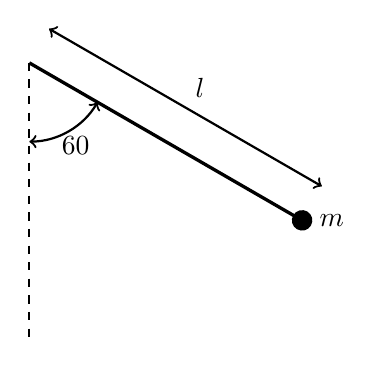
\begin{tikzpicture}
        \draw[thick,dashed](0,0)--(0,-3.5);
        \begin{scope}[rotate=60]
          \draw[very thick](0,0)--(0,-4);
          \fill(0,-4) circle(.13) node[right]{$\;m$};
          \draw[<->,thick](.5,0)--(.5,-4) node[midway,above right]{$l$};
        \end{scope}
        \draw[<->,thick](0,-1)arc(270:330:1)
        node[pos=.6,below]{\ang{60}};
      \end{tikzpicture}
    \end{center}
    \begin{enumerate}[nosep,leftmargin=18pt,label=(\Alph*)]
    \item $\displaystyle T=\frac{1}{2}mg$
    \item $T=mg$
    \item $\displaystyle T=\frac{3}{2}mg$
    \item $T=2mg$
    \item None of the above
    \end{enumerate}
    \vspace{.7in}
    
  \item Two blocks of mass $m_A$ and $m_B$ are connected by a string that
    passes over a light pulley. The mass of $A$ is larger than the mass of $B$.
    The speed of mass $A$ just before reaching the floor is:
    \begin{center}
      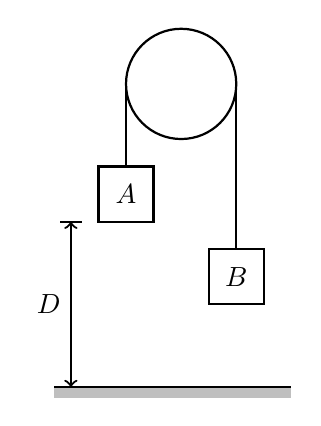
\begin{tikzpicture}[scale=.7]
        \begin{scope}[thick]
          \draw(0,0) circle(1);
          \draw(-1,0)--(-1,-1.5);
          \draw(-1.5,-1.5) rectangle(-.5,-2.5) node[midway]{$A$};
          \draw(1,0)--(1,-3);
          \draw(1.5,-3) rectangle(.5,-4)  node[midway]{$B$};
          \draw(-1.8,-2.5)--(-2.2,-2.5);
          \draw[<->](-2,-2.5)--(-2,-5.5) node[midway,left]{$D$};
          \fill[gray!50](-2.3,-5.7) rectangle(2,-5.5);
          \draw(-2.3,-5.5)--(2,-5.5);
        \end{scope}
      \end{tikzpicture}
    \end{center}
    \begin{enumerate}[nosep,leftmargin=18pt,label=(\Alph*)]
    \item $\displaystyle\sqrt{\frac{2(m_A-m_B)}{m_A+m_B}gD}$
    \item $\displaystyle\sqrt{\frac{2(m_A+m_B)}{m_A-m_B}gD}$
    \item $\displaystyle\sqrt{\frac{2m_A}{m_A+m_B}gD}$
    \item $\displaystyle\sqrt{\frac{2m_B}{m_A+m_B}gD}$
    \item $\displaystyle\sqrt{\frac{2m_A}{m_B}gD}$
    \end{enumerate}
  \end{enumerate}
  \columnbreak
  
  \textbf{Questions \ref{q:down1}--\ref{q:down2}}. A force is applied to a block
  of mass $m$ at a downward angle of $\theta$ to the vertical as shown. The
  block moves with a constant speed across a rough floor for a distance $x$.
  \begin{center}
    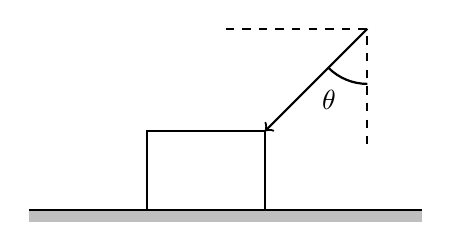
\begin{tikzpicture}
      \fill[gray!50](0,-.15) rectangle(5,0);
      \draw[thick](0,0)--(5,0);
      \draw[thick](1.5,0)rectangle(3,1);
      \draw[<-,thick](3,1)--(4.3,2.3);
      \draw[thick,dashed](2.5,2.3)--(4.3,2.3)--(4.3,.8);
      \draw[thick](4.3,1.6) arc(270:225:.7) node[midway,below left]{$\theta$};
    \end{tikzpicture}

  \end{center}
  \begin{enumerate}[resume,leftmargin=18pt]
  \item The work done by the applied force on the block is
    \label{q:down1}
    \begin{enumerate}[nosep,leftmargin=18pt,label=(\Alph*)]
    \item $Fx\sin\theta$
    \item $Fx\cos\theta$
    \item $Fmx\sin\theta$
    \item $Fmx\cos\theta$
    \item zero
    \end{enumerate}
    
  \item The coefficient of friction between the block and the floor is
    \label{q:down2}
    \begin{enumerate}[nosep,leftmargin=18pt,label=(\Alph*)]
    \item $\displaystyle\frac{F}{mg}$
    \item $\displaystyle\frac{F\cos\theta}{mg}$
    \item $\displaystyle\frac{F\cos\theta}{F\sin\theta+mg}$
    \item $\displaystyle\frac{F\sin\theta}{F\cos\theta+mg}$
    \item $\displaystyle\frac{F\cos\theta}{F\sin\theta}$
    \end{enumerate}
  \end{enumerate}
  
  \textbf{Questions \ref{sphere1}--\ref{sphere2}}. A small block rests on the
  top of a smooth sphere of radius $R$ when it is given a light tap so that it
  just begins sliding on the sphere. When the block reaches the angle $\theta$,
  it loses contact with the surface of the sphere.
  \begin{center}
    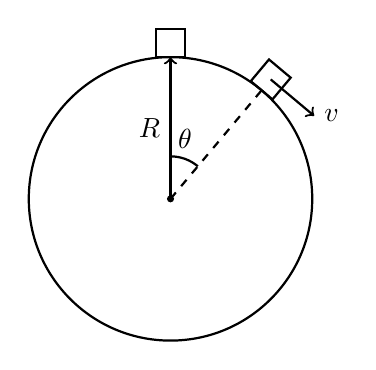
\begin{tikzpicture}[scale=.9]
      \draw[thick](0,0) circle(2);
      \fill(0,0) circle(.05);
      \draw[thick,->](0,0)--(0,2) node[midway,left]{$R$};
      \draw[thick](-.2,2) rectangle(.2,2.4);
      \begin{scope}[rotate around={-40:(0,0)}]
        \draw[thick,dashed](0,0)--(0,2);
        \draw[thick](-.2,2) rectangle(.2,2.4);
        \draw[->,thick](0,2.2)--(.8,2.2) node[right]{$\mb{v}$};
      \end{scope}
      \draw[thick](0,.6) arc(90:50:.6) node[midway,above]{$\theta$};
    \end{tikzpicture}
  \end{center}  
  \begin{enumerate}[resume,leftmargin=18pt]
  \item The kinetic energy of the block as it leaves the surface of the sphere
    is
    \label{sphere1}
    \begin{enumerate}[nosep,leftmargin=18pt,label=(\Alph*)]
    \item $mgR$
    \item $mgR\cos\theta$
    \item $mgR\sin\theta$
    \item $mg(R-R\cos\theta)$
    \item $mg(R-R\sin\theta)$
    \end{enumerate}

  \item The speed of the block as it leaves the surface of the sphere is
    \label{sphere2}
    \begin{enumerate}[nosep,leftmargin=18pt,label=(\Alph*)]
    \item $\displaystyle\sqrt{2g}{m}$
    \item $\displaystyle\sqrt{2gR}{m}$
    \item $\displaystyle\sqrt{2gR\cos\theta}$
    \item $\displaystyle\sqrt{2g(R-R\cos\theta)}$
    \item $\displaystyle\sqrt{2g(R-R\sin\theta)}$
    \end{enumerate}
    
  \item A machine can lift large weights according to the power equation
    $P(t)=4t^3+3t^2-2$, where power is in watts and time is in seconds. The
    energy expended by the machine from $t=0$ to $t=\SI{10}{\second}$ is
    \begin{enumerate}[nosep,leftmargin=18pt,label=(\Alph*)]
    \item\SI{1260}{\joule}
    \item\SI{3630}{\joule}
    \item\SI{9240}{\joule}
    \item\SI{10980}{\joule}
    \item\SI{18150}{\joule}
    \end{enumerate}
    
  \item A small ball starts from rest and rolls down a quarter-circle ramp of
    radius $R$. The speed of the ball at the point halfway down the ramp is
    most nearly
    \begin{center}
      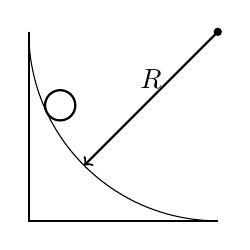
\begin{tikzpicture}[scale=2.4]
        \draw[thick](-1,0)--(-1,-1)--(0,-1);
        \draw(-1,0) arc(180:270:1);
        \draw[thick,->,rotate=45](0,0)--(-1,0) node[midway,above,sloped]{$R$};
        \draw[thick,rotate=25](-.92,0) circle(.08);
        \fill (0,0) circle(.022);
      \end{tikzpicture}
    \end{center}
    \begin{enumerate}[nosep,leftmargin=18pt,label=(\Alph*)]
    \item $gR$
    \item $2gR$
    \item $\displaystyle\sqrt{gR\sin\ang{45}}$
    \item $\displaystyle\sqrt{2gR\sin\ang{45}}$
    \item The speed cannot be determined without knowing the mass of the ball.
    \end{enumerate}
  \end{enumerate}
\end{multicols}
\newpage

\genfreetitle{C}{WORK AND ENERGY}{6}

\genfreedirections

\begin{enumerate}[leftmargin=15pt]

\item A mass $m$ is placed on an incline of angle $\theta$ at a distance $d$
  from the end of a spring as shown below. The coefficient of kinetic friction
  between the mass and the plane is $\mu$.
  \cpic{.3}{ramp1}
  \begin{enumerate}
  \item The mass is released from rest at the position shown. Using Newton's
    laws, calculate the block's speed when it reaches the spring.
  \item Using energy conservation, alculate the block's speed when it reaches
    the spring.
  \item The spring has spring constant $k$. At what value $x$ of the compression
    of the spring does the object reach its maximum speed?
  \end{enumerate}
  \newpage
  
\item A mass $m$ attached to a string of length $2r$ swings, starting at rest
  when the string is horizontal, until the string is vertical. At the instant
  the string is vertical, the mass makes contact with the horizontal surface,
  the string is cut, and the mass continues along a frictionless track as shown
  below.
  \begin{center}
    \vspace{-.1in}
    \begin{tikzpicture}[scale=1.5]
      \begin{scope}[thick]
        \draw(0,0)--(-2,0);
        \draw[<->](0,.25)--(-2,.25) node[midway,above]{$2r$};
        \draw(-2,.1) rectangle (-2.3,-.1) node[midway]{$m$};
        \draw[->](-2.15,-.15) arc(185:200:2.15);
        \draw[dashed](0,0)--(0,-2);
        \draw(-.7,-2)--(2.5,-2);
        \draw (2.5,-2) arc(-90:90:1);
        \fill(2.5,-1) circle(.05);
        \draw[rotate around={40:(2.5,-1)},->] (2.5,-1)--(3.5,-1)
        node[midway,above]{$r$};
      \end{scope}
    \end{tikzpicture}
  \end{center}
  \begin{enumerate}[leftmargin=18pt]
  \item What is the speed of the mass attached to the string the instant the
    string is cut?
    \vspace{\stretch1}
  \item Sketch the forces acting on the mass when it is in the position shown
    below.
    \begin{center}
      \begin{tikzpicture}[scale=2]
        \begin{scope}[thick]
        \draw(0,-2)--(2.5,-2);
        \draw (2.5,-2) arc(-90:90:1);
        %\fill(2.5,-1) circle(.05);
        \begin{scope}[rotate around={40:(2.5,-1)}]
          \draw[dashed](2.5,-1)--(3.5,-1);
          \draw[fill=gray!50](3.5,-.93) rectangle (3.36,-1.07);
        \end{scope}
        \draw[dashed](2.5,-1)--(2.5,0);
        \draw(2.5,-.6) arc(90:40:.4) node[midway,above]{$\theta$};
        \end{scope}
    \end{tikzpicture}
    \end{center}
  \end{enumerate}
  When the mass is in the position shown above,
  \begin{enumerate}[resume]
  \item Find the object's speed as a function of $\theta$
  \item Find the object's centripetal acceleration as a function of $\theta$
  \item Determine at what angle $\theta$ the mass will fall of the track
  \end{enumerate}
  \vspace{\stretch1}
  \newpage

  % TAKEN FROM THE 2009 AP PHYSICS C EXAM FREE-RESPONSE QUETION MECH 1
\item A \SI{3.}{\kilo\gram} object is moving along the $x$-axis in a region
  where its potential energy as a function of $x$ is given as $U(x)=4.0x^2$,
  where $U$ is in joules and $x$ is in meters. When the object passes the point
  $x=\SI{-0.50}{\metre}$, its velocity is $+$\SI{2.}{\metre\per\second}. All
  forces acting on the object are conservative.
  \begin{enumerate}[leftmargin=18pt]

  \item Calculate the total mechanical energy of the object.
  \item Calculate the $x$-coordinate of any points at which the object has zero
    kinetic energy.
  \item Calculate the magnitude of the momentum of the object at
    $x=\SI{.60}{\metre}$.
  \item Calculate the magnitude of the acceleration of the object as it passes
    $x=\SI{.60}{\metre}$.
  \item On the axes below, sketch graphs of the object's position $x$ versus
    time $t$ and kinetic energy $K$ versus time $t$. Assume that $x=0$ at time
    $t=0$. The two graphs should cover the same time interval and use the same
    scale on the horizontal axes.
    \begin{center}
      \begin{tikzpicture}
        \draw[very thick,->](-1,0)--(10,0)node[right]{$t$};
        \draw[very thick,->](0,-3)--(0,3)node[above]{$x$};
      \end{tikzpicture}
      \vspace{.2in}
      \begin{tikzpicture}
        \draw[very thick,->](-1,0)--(10,0)node[right]{$t$};
        \draw[very thick,->](0,-3)--(0,3)node[above]{$K$};
      \end{tikzpicture}
    \end{center}
  \end{enumerate}
  
%\item The theoretical formula for the potential energy associated with the
%  nuclear force between two protons, two neutrons, or a proton and a neutron
%  is the \emph{Yukawa potential}:
%  \begin{displaymath}
%    U=-U_0\left(\frac{a}{x}\right)e^{-x/a}
%  \end{displaymath}
%  where $U_0$ and $a$ are constants.
%  \begin{enumerate}[noitemsep]
%  \item Sketch $U$ versus $x$ using $U_0=\SI{4}{\pico\joule}$ and
%    $a=\SI{2.5}{\femto\metre}$.
%  \item Find the force $F_x$.
%  \item Compare the magnitude of the force at the separation $x=2a$ to that at
%    $x=a$.
%  \item Compare the magnitude of the force at the separation $x=5a$ to that at
%    $x=a$.
%  \end{enumerate}
%  \vspace{\stretch{1}}
  \newpage
  
\item A small block of mass $m$ slides without friction along the loop-the-loop
  track shown in the figure. The block starts from point $P$ a distance $h$
  above the bottom of the loop.
  \begin{center}
    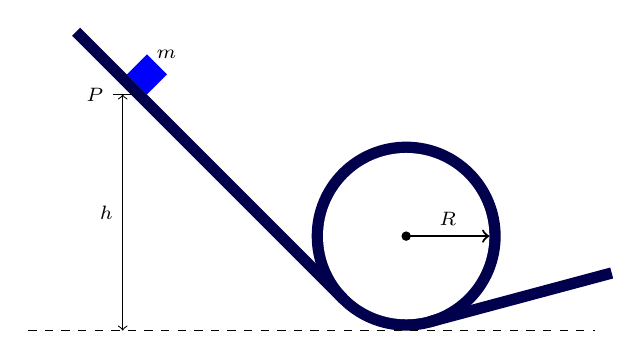
\begin{tikzpicture}[scale=1.2]
      \fill[blue!30!black](0,0) circle(1);
      \fill[white](0,0) circle(.88);
      \fill(0,0) circle(.05);
      \draw[thick,->](0,0)--(.88,0)node[midway,above]{\scriptsize$R$};
      \draw[dashed](-4,-1)--(2,-1);
      \fill[rotate=15,blue!30!black](0,-1)rectangle(2,-.88);
        \begin{scope}[rotate=-45]
          \fill[blue!30!black](0,-1)rectangle(-4,-.88);
          \fill[blue](-3,-.88)rectangle(-3.3,-.58)
          node[black,right]{\scriptsize$m$};
        \end{scope}
        \draw[<->](-3,-1)--(-3,1.5) node[midway,left]{\scriptsize$h$};
        \draw(-2.9,1.5)--(-3.1,1.5) node[left]{\scriptsize$P$};
    \end{tikzpicture}
  \end{center}
  \begin{enumerate}[nosep]
  \item What is the kinetic energy of the block when it reaches the top of
    the loop?
  \item What is the acceleration at the top of the loop, assuming that it
    stays on the track?
  \item What is the least value of $h$ for which the block will reach the top
    of the loop without leaving the track?
  \end{enumerate}
  \newpage

\item A pendulum of length $L$ has a bob of mass $m$. It is released from some
  angle $\theta_1$. The string hits a peg at a distance $x$ directly below the
  pivot, as shown in the figure below, effectively shortening the length of the
  pendulum. Find the maximum angle $\theta_2$ between the string and the
  vertical when the bob is to the right of the peg.
  \begin{center}
    \pic{.4}{pendulum-peg}
  \end{center}
  \vspace{\stretch1}
  \newpage
  
\item A \SI{2.}{\kilo\gram} block $m$ is released \SI{4.}{\metre} from a
  massless
  spring with a spring constant of $k=\SI{100}{\newton\per\metre}$ that is fixed
  along a frictionless plane inclined at \ang{30}, as shown in the figure below.
  (Plese give answer to $3$ significant figures.)
  \begin{center}
    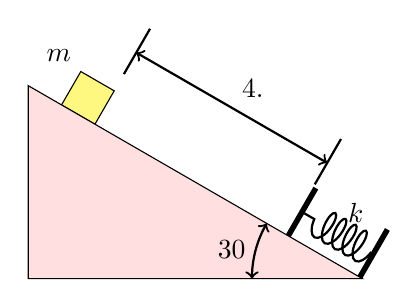
\begin{tikzpicture}[scale=.7]
      \begin{scope}[rotate=-30]
        \fill(0,0) rectangle(-.1,1);
        \draw[thick,
          decoration={aspect=.4,segment length=1.5mm, amplitude=2mm,coil},
          decorate] (-.1,.5)--(-1.5,.5)
        node[midway,above right]{$k$};
        \fill(-1.5,0) rectangle(-1.6,1);
        \draw[<->,thick](-1.6,1.5)--(-5.6,1.5)
        node[midway,above right,sloped]{\SI{4.}{\metre}};
        \draw[thick](-1.6,1.05)--(-1.6,2);
        \draw[thick](-5.6,1.05)--(-5.6,2);
        \draw[fill=yellow!50](-5.6,0) rectangle(-6.3,.7)
        node[black,above left]{$m$};
      \end{scope}
      \draw[fill=pink!50](0,0)--(-6.06,0)--(-6.06,3.5)--cycle;
      \draw[<->,thick](-2,0) arc(180:150:2) node[midway,left]{\ang{30}};
    \end{tikzpicture}
  \end{center}
  \begin{enumerate}[noitemsep,leftmargin=20pt]
  \item Find the maximum compression of the spring.
  \item If the plane is not frictionless, and the coefficient of kinetic
    friction between it and the block is $\mu=0.20$, find the maximum
    compression.
  \item For the rough incline ($\mu=0.20$), how far up the incline will the
    block travel after leaving the spring?
  \end{enumerate}
\end{enumerate}
\end{document}
